\documentclass[a4paper,11pt]{article}
\usepackage{a4wide}
\usepackage{fullpage}
\usepackage[utf8x]{inputenc}

\usepackage[light,math]{anttor}
\usepackage[T1]{fontenc}

%\usepackage[slovene]{babel}
%\selectlanguage{slovene}
\usepackage[toc,page]{appendix}
\usepackage[pdftex]{graphicx} 

\usepackage{lmodern}
\usepackage{amsmath}
\usepackage{amssymb}
\usepackage{amsthm}
\usepackage{amsfonts}
\usepackage{mathtools}
\usepackage{enumitem}
\usepackage{amsfonts}
\usepackage{setspace}
\usepackage{color}
\definecolor{light-gray}{gray}{0.95}
\usepackage{listings} 
\usepackage{hyperref}
\usepackage[english, croatian, slovene]{babel}

\renewcommand{\baselinestretch}{1.2} 
\renewcommand{\appendixpagename}{Priloge}


\title{Algoritmi \\
\textbf{Domača naloga 3} }
\author{Sara Bizjak  |  27202020}
\date{April 2021}

%%%%%%%%%%%%%%%%%%%%%%%%%%%%%%%%%%%%%%%%%%%%%%%%%%%%%%%%%%%%%%%%%%%%%%%%%%%%%%%%%%%%%%%%%%%%%%%%%%%%%%%%%%%%%%%%%%%%%%%%%%%%%%%%%

\begin{document}

\maketitle

%%%%%%%%%%%%%%%%%%%%%%%%%%%%%%%%%%%%%%%%%%%%%%%%%%%%%%%%%%%%%%%%%%%%%%%%%%%%%%%%%%%%%%

\section*{Problem 1 - Konveksna ovojnica}

\noindent
Naj bosta $S_1$ in $S_2$ konveksni ovojnici v ravnini. 

\subsection*{A del:} Algoritem za izračun unije teh dveh ovojnic.

\subsection*{B del:} Algoritem, ki preveri, če se konveksni ovojnici sekata.
%%%%%%%%%%%%%%%%%%%%%%%%%%%%%%%%%%%%%%%%%%%%%%%%



%%%%%%%%%%%%%%%%%%%%%%%%%%%%%%%%%%%%%%%%%%%%%%%%%%%%%%%%%%%%%%%%%%%%%%%%%%%%%%%%%%%%%%%%%%%%%%%%

\section*{Problem 2 - Delaunay triangulacija}
Podan imamo naključnosti algoritem za iskanje Delaunay triangulacije (opisan v \cite{delaunay}) s pričakovanim časom izvajanja $\mathcal{O}(n \log n)$. Pokažemo, da je najslabši čas izvajanja $\mathcal{O}(n^2)$.
\\
\\
Zgeneriramo primer, pri katerem se za vsako dodano točko $p_i$ v $i$-item koraki generira okoli $i$ novih robov (z \textit{edge flipping-om}).
\\
Opazujmo množico $n$ točk $P$, ki leži na pozitivni veji parababole $y = x^2$, torej
\begin{align*}
    P = \{ (t_1, t_1^2), (t_2, t_2^2), \ldots , (t_n, t_n^2)\},
\end{align*}
kjer so $t_1, t_2, \ldots t_n$ pozitivna realna števila. BŠS predpostavimo $0 < t_1 < \cdots < t_n$.
\\
Trdimo, da je v Delaunay triangulaciji $P$-ja najbolj leva točka $(t_1, t_1^2)$ sosednja z vsako drugo točko iz $P$. To pomeni, da z dodajanjem vsake nove točke $(t_0, t_0^2)$ v $P$, tako da velja $0 < t_0 < t_1$ (torej bo ta na novo dodana točka najbolj leva), generiramo tudi $n$ novih robov Delaunay triangulaciji. 
Če torej dodajamo točke od desne proti levi, je število robov v Delaunayevi triangulaciji enako $\Omega(n^2)$.
\\
\\
\textit{Dokaz.} \\
Naj bodo $0 < a < b < c$ pozitivna realna števila in naj bo $\mathcal{C}(a, b, c)$ krožnica skozi točke $(a, a^2), (b, b^2), (c, c^2)$, ki tvorijo trikotnik v triangulaciji.
\\
Trdimo, da $\mathcal{C}(a, b, c)$ ne vsebuje nobene take točke $d$, kjer
\begin{align*}
    a < d < b \ \text{ali} \ c < d
\end{align*} 
Pokažimo to s protislovjem in recimo, da točka $(d, d^2)$ leži na krožnici $\mathcal{C}(a, b, c)$. To je natanko tedaj, ko velja
\begin{align*}
    \begin{vmatrix}
        1 & a & a^2 & a^2 + a^4 \\
        1 & b & b^2 & b^2 + b^4 \\
        1 & c & c^2 & c^2 + c^4 \\
        1 & d & d^2 & d^2 + d^4 \\
    \end{vmatrix}
    = 0,
\end{align*}
kar je enako pogoju
\begin{align*}
    (a - b)(a - c)(b - c)(a - d)(b - d)(c - d)(a + b + c + d) = 0.
\end{align*}
Od tukaj sledi, da mora veljati ena od zvez
\begin{align*}
    d &= a \\
    d &= b \\
    d &= c \\
    d &= - a - b - c < 0,
\end{align*}
saj iz $(a - b), (a - c), (b - c)$ ne moremo dobiti ničle, ker $0 < a < b < c$.
Velja tudi, da $(a - d) \neq (b - d) \neq (c - d) \neq (a + b + c + d)$, kar pomeni, da parabola dejansko seka krožnico $\mathcal{C}(a, b, c)$ v teh štirih točkah. 
Iz tega sledi, da točka $(d, d^2)$ leži znotraj krožnice $\mathcal{C}(a, b, c)$, če velja
\begin{align*}
    - a - b - c < d < a  \ 
    \text{ali}
    \ 
    b < d < c
\end{align*}    
Sklepi nam podajo protislovje.
\\
Če torej dodajamo točke, kot je opisano v primeru, je časovna zahtevnost algoritma res s$\Omega(n^2)$.
%%%%%%%%%%%%%%%%%%%%%%%%%%%%%%%%%%%%%%%%%%%%%%%%%%%%%%%%%%%%%%%%%%%%%%%%%%%%%%%%%%%%%%%%%%%%%%%%

\section*{Problem 3 - Iskanje točk s kd, četrtinskimi in intervalnimi drevesi}

\subsection*{A del:}
Kd-drevesa, četrtinska drevesa in intervalna drevesa so podatkovne strukture za hranjenje množice točk v ravnini. 
Vsaka izmed teh struktur ima dotično prednost pred ostalimi pri določenih pogojih.

\begin{itemize}
    \item \textit{Kd-drevo -- linearna prostorska zahtevnost $\mathcal{O}(n)$.} Prostorska zahtevnost intervalnih dreves je $\mathcal{O}(n \log^{d - 1}(n))$, kjer je $n$ število shranjenih točk v drevesu, $d$ pa njihova dimenzija, četrtinskih pa $\mathcal{O}((g + 1) n)$. Tukaj z $g$ označimo globino drevesa, ki pa je logaritemsko odvisna od razmerja med najmanjšo razdaljo med dvema točkama in stranico začetnega kvadrata. Ker je v teoriji tako razmerje lahko poljubno, je lahko potem tudi prostorska zahtevnost poljubna (velika). 
    \item \textit{Četrtinsko drevo -- dodajanje novih točk v že zgrajeno drevo.} Če v že zgrajeno drevo dodamo nove točke, se četrtinsko drevo ne bo spremenilo, medtem ko sta lahko po dodajanju kd-drevo in intervalno drevo precej spremenjeni in drugačni, kot če bi imela že na začetku na razpolago vse točke.
    \item \textit{Intervalno drevo -- hitrejše poizvedbe.} Iskanje v intervalnem drevesu je navzgor omejeno z $\mathcal{O}(\log^d n)$, iskanje v kd-drevesu poteka v $\mathcal{O}(n)$. V primerjavi s četrtinskim drevesom pa ima boljši čas za iskanje tuidi v primerih, ko so točke manj ugodno razporejene. Taka razporeditev je opisana v prvi alineji.
\end{itemize}
    
\subsection*{B del:}
Naj bo $P$ množica točk v $3$-dimenzionalnem prostoru. Opišemo algoritem za izdelavo osmiškega drevesa točk iz $P$.
\\
Vhod algoritma je množica točk $P$. Če začetne kocke nimamo podane, jo izračunamo s pomočjo ekstremov v vseh treh smereh, tj. v $x$, $y$ in $z$ smeri, saj smo v $3$-dimenzionalnem prostoru.
\\
Ko imamo začetno kocko določeno, algoritem ponavljamo rekurzivno. 
Če je v kocki več kot ena točka, jo razdelimo na osem enako velikih delov (oktantov), ki predstavljajo otroke kocke, ki smo jo razdelili.
Enako ponavljamo na otrocih z več kot eno vsebovano točko. Algoritem zaključi in vrne osmiško drevo, ko v nobenem delu ni več kot ene točke. 





%%%%%%%%%%%%%%%%%%%%%%%%%%%%%%%%%%%%%%%%%%%%%%%%%%%%%%%%%%%%%%%%%%%%%%%%%%%%%%%%%%%%%%%%%%%%%%%%

\newpage
\begin{thebibliography}{99}
    \bibitem{delaunay}
    Mark De Berg, Marc Van Kreveld, Mark Overmars, and Otfried CheongSchwarzkopf.    Computational  geometry.    In \emph{Computational  geometry}, pages 1–17. Springer, 2000.

    \bibitem{clanek}
    Don Sheehy, \emph{Computational Geometry: Lecture 7}, 2010, [ogled 15.~4.~2021], dostopno na
    \url{www.cs.cmu.edu/afs/cs/academic/class/15456-s10/ClassNotes/lecture7.pdf}

\end{thebibliography}
    
\end{document}

Za Delanuayevo triangulacijo velja:
\\
\textit{Definicija.} Naj bo $T(S)$ triangulacija na $S$ in naj bo $ab$ deljen rob trikotnikov $abc$ in $abd$ v $T(S)$. Rob $ab$ je lokalno Delaunayev (v nadaljevanju [LD]), če $d \notin Int \mathcal{C}(a, b, c)$.
\\
\begin{figure}[ht!]
    \center
    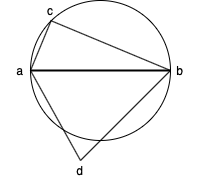
\includegraphics[width = 55mm]{LD.png}
    \caption{Pogoj, da je rob $ab$ [LD].}\label{pic:ld}
\end{figure}

\noindent
\textit{Definicija.} Triangulacija je Delanuayeva, če in samo če je vsak rob [LD].
\\
Algoritem za iskanje Delanuay triangulacije tedaj poteka na sledeč način:
\begin{enumerate}
    \item Začnemo s katerokoli triangulacijo.
    \item Za vsak rob preverimo ali je [LD]. Če rob ni [LD], ga obrnemo (\textit{angl. flipping}).
\end{enumerate}
Vprašanje je, kako preverimo, če je rob v triangulaciji [LD]. Ker za [LD] ne sme veljati, da četrta točka (označena z $d$) leži v krožnici, konstruirani skozi prve tri točke (označene z $a, b, c$), potrebujemo kriterij za preverjanje omenjenega pogoja, predstavljenega tudi na sliki \ref{pic:ld}.

%%%%%%%%%%%%%%%%%%%%%%%%%%%%
%%%%%%%%%%%%%%%%%%%%%%%%%%%%


Opazujmo množico $n$ točk $P$, ki leži na pozitivni veji parababole $y = x^2$, torej
\begin{align*}
    P = \{ (t_1, t_1^2), (t_2, t_2^2), \ldots , (t_n, t_n^2)\},
\end{align*}
kjer so $t_1, t_2, \ldots t_n$ pozitivna realna števila. BŠS predpostavimo $0 < t_1 < \cdots < t_n$.
\\
Trdimo, da je najbolj leva točka $(t_1, t_1^2)$ sosednja z vsako drugo točko iz $P$. To pomeni, da z dodajanjem vsake nove točke $(t_0, t_0^2)$ v $P$, tako da velja $0 < t_0 < t_1$ (torej bo ta na novo dodana točka najbolj leva), dodamo tudi $n$ novih robov Delaunay triangulaciji. 
Če torej dodajamo točke od desne proti levi, je število robov v Delaunayevi triangulaciji enako $\Omega(n^2)$.
\\
\\
Naj bodo $0 < a < b < c$ pozitivna realna števila in naj velja in naj bo $\mathcal{C}(a, b, c)$ krožnica skozi točke $(a, a^2), (b, b^2), (c, c^2)$, ki tvorijo trikotnik v triangulaciji.
\\
Trdimo, da $\mathcal{C}(a, b, c)$ ne vsebuje nobene take točke $d$, kjer
\begin{align}\label{protislovje1}
    a < d < b \ \ \ \text{ali} \ \ \  c < d
\end{align} 
Pokažimo to s protislovjem in recimo, da točka $(d, d^2)$ leži znotraj krožnice $\mathcal{C}(a, b, c)$. To je natanko tedaj, ko velja
\begin{align*}
    \begin{vmatrix}
        1 & a & a^2 & a^2 + a^4 \\
        1 & b & b^2 & b^2 + b^4 \\
        1 & c & c^2 & c^2 + c^4 \\
        1 & d & d^2 & d^2 + d^4 \\
    \end{vmatrix}
    = 0,
\end{align*}
kar je enako pogoju
\begin{align*}
    (a - b)(a - c)(b - c)(a - d)(b - d)(c - d)(a + b + c + d) = 0.
\end{align*}
Od tukaj sledi, da mora veljati ena od zvez
\begin{align*}
    t &= a \\
    t &= b \\
    t &= c \\
    t&= - a - b - c < 0,
\end{align*}
saj iz $(a - b), (a - c), (b - c)$ ne moremo dobiti ničle, ker $0 < a < b < c$.
Velja tudi, da $(a - d) \neq (b - d) \neq (c - d) \neq (a + b + c + d)$, kar pomeni, da parabola dejansko seka krožnico $\mathcal{C}(a, b, c)$ v teh štirih točkah. 
Iz tega sledi, da točka $(d, d^2)$ leži znotraj krožnice $\mathcal{C}(a, b, c)$, če velja
\begin{align}\label{protislovje2}
    - a - b - c < d < a  \ \ \ 
    \text{ali}
    \ \ \ 
    b < d < c
\end{align}    
Pogoja \ref{protislovje1} in \ref{protislovje2} nam podata protislovje.